% Schematic of cloud and terrain parallax (scripts/make_paper_figures.py, fig0_schematic).
\begin{figure}[tbp]
  \centering
  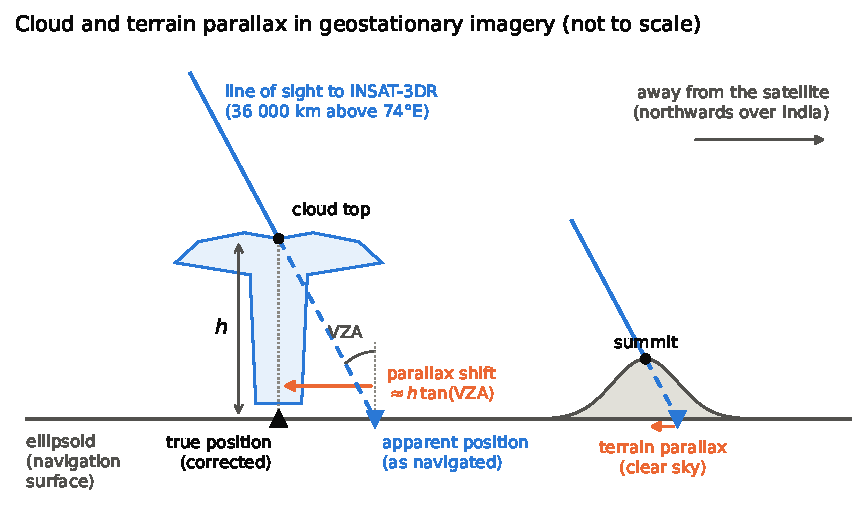
\includegraphics[width=\textwidth]{figures/fig0_schematic.pdf}
  \caption{Cloud and terrain parallax in geostationary imagery (cross-section, not to scale). A cloud top at height $h$ is seen along the line of sight from the satellite and is navigated to where that line meets the ellipsoid (apparent position), displaced away from the satellite by about $h\tan(\mathrm{VZA})$. The correction moves it back to the point on the line of sight at height $h$ (true position). Elevated terrain is displaced in the same way in clear sky.}
  \label{fig:schematic}
\end{figure}
